%! Mode:: "TeX:UTF-8"
%! TEX program = xelatex
\PassOptionsToPackage{quiet}{xeCJK}
\documentclass[withoutpreface,bwprint]{thesis-config}
\usepackage{third}

\begin{document}
\maketitlepage{智能图书馆派送路径优化}{周意尧、樊铧纬、戴承江、杨逍宇}{\today}{何衍} %封面页 



\begin{abstract}

\par \textbf{对于问题一},我们采用贪心算法来解决智能机器人在图书馆进行派送任务时的路径规划问题。目标是规划其运动路径,使其行驶路径最短。通过建立相应的数学模型,并考虑每个途径点只能访问一次等约束条件,我们直接利用贪心算法进行求解,得出最优路径,提升了AGV的取书效率。
\par \textbf{对于问题二},针对多AGV智能机器人同时取书的场景,我们将此问题建模为SDVRP(Split Delivery Vehicle Routing Problem)问题。通过贪婪算法和蚁群算法的结合,解决了多辆AGV的协同调度问题,确保每个机器人在载满书籍或未取满情况下合理返回传送处,最终求解出总行驶路径最短的调度方案。
\par \textbf{对于问题三},提出了一种基于混合整数规划(MILP)的方法,用于解决仓储环境中托盘与书籍的高效拣选和调度问题。我们建立了一个详细的数学模型,考虑了托盘内书本数量与预约订单匹配、托盘与书籍挑选节点的匹配、托盘放回空储位节点以及空托盘回收等多个约束条件。通过定义变量和约束条件,模型确保了从托盘中挑选出的书籍数量满足预约订单需求,同时最小化了托盘在仓库中的移动距离。模型的主要约束包括:托盘内书本数量与预约订单匹配约束、托盘与书籍挑选节点的匹配约束、托盘与回收处和储位的约束。


\keywords{智能机器人\quad 贪心算法\quad 遗传算法\quad SDVRP \quad MILP}
\begin{figure}[!htbp]
    \centering
    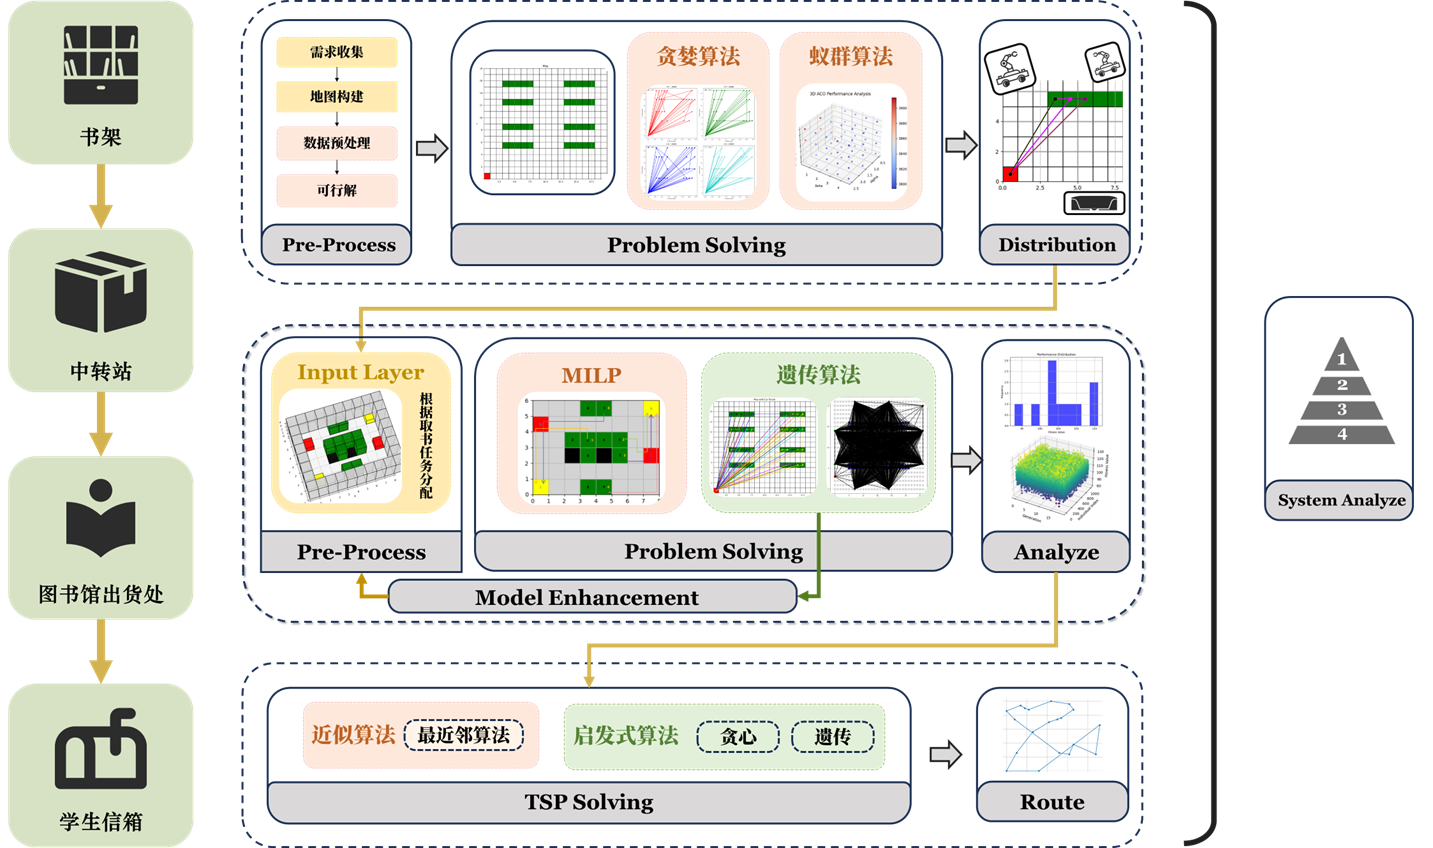
\includegraphics[width=1\linewidth]{figures/structue.png}
\end{figure}
\end{abstract}


\tableofcontents  % 目录
\newpage

\section{问题描述}
\subsection{问题背景}
\par 在这样一个全民阅读的时代,国民人均阅读量不断增加,人们对便捷、高效的借阅服务需求也与日俱增。为了满足这一需求,浙江大学在去年又开了一座新的主图书馆,并引入先进的智能机器人技术,为读者提供更方便的借阅条件。该系统采用“网上预定——自动分拣——送书上门”的一条龙服务模式,读者只需在手机端预约心仪的书籍,系统便会根据预约时间将书籍分配到不同的托盘中。AGV智能机器人会根据预设的路线,将装载书籍的托盘从储位搬运到拣选工位,完成书籍的打包,最后将包裹送至读者的指定地点。这种新型的借阅模式,不仅能有效地提高图书馆资源的利用率和服务效率,还能为读者提供更加便捷、人性化的借阅体验,并极大地提升图书馆的服务水平,为推动全民阅读做出积极贡献。
\par 本任务总共分为三个步骤:
\par \textbf{1.书籍挑选}
\par 同学在手机通过浙大钉的图书馆应用可以进行线上借阅,在收到预约订单之后,我们规定,在每天的固定时间11点和8点对于该点之前的预约信息进行处理,即将预约书籍从货架上挑选出来,放在托盘中,然后送往传送处,最后送往书籍发货处。(注:在该取书情况下,不同时间处理的订单将会储存在不同的托盘中)
\par \textbf{2.书籍送货}
\par 在书籍通过托盘送到发货处的货架上时,机器人会在每天的13点进行处理,订单一次处理50单(考虑到每天预约书籍的量并没有那么多而设置的),处理订单的步骤分为三步。
\par \quad (1) AGV搬运载有书本的托盘到空闲拣选工位;
\par \quad (2) AGV搬运拣选完成的托盘从工位回到仓库内空储位;
\par \quad (3) AGV搬运拣选完成的空托盘从工位到托盘回收处;
\par 对于该问题来说,我们认为每一本书就是一个订单,不考虑多本书一起打包发送这件事情
\par \textbf{3.派送到户}
\par 小车将已经打包好的书籍送往每一位同学的信箱中。
%%%%%%%%%%%%%%%%%%%%%%%%%%%%%%%%%%%%%%%%%%%%%%%%%%%%%%%%%%%%% 

\subsection{问题提出}
\par \textbf{问题1:送书小车统筹调度问题}  
\par 现在智能小车要进行派送任务,已知其要经过的途径点,请你规划其运动路径使其经过所有途径点并使行驶路径最短。
\par \textbf{问题2:取书AGV统筹调度问题}  
\par 考虑4辆AGV智能机器人同时取书,机器人从起始位置出发,然后前往书架取书了,每一个机器人一次最多承载5本书,一旦取了5本书之后,必须前往传送处将书放下,再回去取书(机器人可以自行决定装载几本书后前往传送处,即未取满8本书也可放回传送处),请你规划4个机器人的路径使得其总行驶路径最短。
\par \textbf{问题3:AGV指派调度问题}  
\par AGV智能机器人从起始位置出发,先前往储位取下装有预定订单中书籍的托盘,然后送往挑选处将订单中需要的书籍挑选出去,挑选完成之后,如果托盘中没有书籍,则前往托盘回收处,如果仍然有书籍,则将托盘送回货架上,任务到此结束。不考虑小车完成任务后回到出发点的这一段距离,请你指派小车和托盘,使得AGV智能机器人取托盘以及托盘运行总路径长度最短。



%%%%%%%%%%%%%%%%%%%%%%%%%%%%%%%%%%%%%%%%%%%%%%%%%%%%%%%%%%%%% 
\section{问题分析}
\subsection{问题一分析}
对于问题一,这是一个TSP旅行商问题,我们建立了相应的数学模型,考虑每个城市必须被访问仅一次、从起点出发最后回到起点等约束条件,考虑到图书馆的派送任务不算复杂我们直接利用贪心算法进行求解。
\begin{figure}[!htbp]
    \centering
    
\includegraphics[width=0.5\linewidth]{figures/str-1.png}
\end{figure}
\subsection{问题二分析}	
对于问题二,这个SDVRP(Split Delivery Vehicle Routing Problem)属于组合优化问题(Combinatorial Optimization Problem),我们采用贪婪算法和蚁群算法来解决取书AGV统筹调度问题。我们建立了一个详细的数学模型,考虑了运输小车给书架的配送量和书架需求量的匹配,考虑运输小车容量的约束,考虑运输支路限制条件等多个约束条件。过定义变量和约束条件,模型确保了从运输小车的运输总量满足预约订单需求,同时最小化了运输小车在图书馆取数过程中的移动距离。
\begin{figure}[!hbtp]
    \centering
    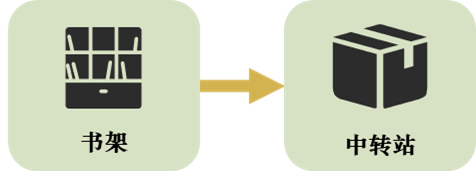
\includegraphics[width=0.5\linewidth]{figures/str-2.png}
\end{figure}
\subsection{问题三分析}	
对于问题三,提出了一种基于混合整数规划(MILP)的方法,用于解决仓储环境中托盘与书籍的高效拣选和调度问题。我们建立了一个详细的数学模型,考虑了托盘内书本数量与预约订单匹配、托盘与书籍挑选节点的匹配、托盘放回空储位节点以及空托盘回收等多个约束条件。通过定义变量和约束条件,模型确保了从托盘中挑选出的书籍数量满足预约订单需求,同时最小化了托盘在仓库中的移动距离。可以先通过对小规模数据的实验,证明模型能够有效地最小化总路程,并确保所有书籍被正确拣选。再进一步扩展到大规模数据,并使用更大的地图进行实验。
\begin{figure}[!htbp]
    \centering
    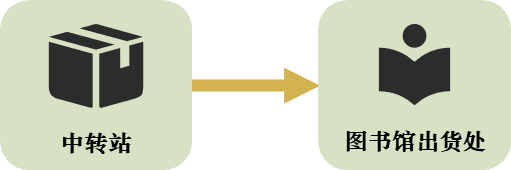
\includegraphics[width=0.5\linewidth]{figures/str-3.png}
\end{figure}
\section{模型假设}

\par 为简化问题,本文做出以下假设:

\begin{itemize}[itemindent=2em]
\item 假设1:对于所有问题,不考虑机器人的实际体积可能造成的碰撞问题
\item 假设2:对于问题二,我们假设一个货架只能储存一个托盘来存放书籍
\item 假设3:对于问题二,我们只考虑完成取书——挑拣——回收/放回这一任务的最短距离,不考虑AGV小车的调度问题,即不考虑多辆小车的调度问题
\end{itemize}
\section{符号说明}

\begin{table}[H]
	\centering
	\begin{tabular}{c c c}
		\toprule
		\makebox[0.3\textwidth][c]{符号}	&  \makebox[0.4\textwidth][c]{说明} \\ \hline
        $N$ & 有需要取书的书架的数量\\
        $C$ & 运输小车的数量\\
        $d_{ij}$ & 书架$i$和书架$j$之间的距离\\
        $Q$ & 运输小车的装载容量\\
        $x_{ijk}$ & 运输小车$k$是否通过边($i,j$)的二进制标识符\\
        $y_{ik}$  & 运输小车$k$在书架$i$的配送数量\\
        $q_i$ & 第$i$个书架的需求量\\
        $s$ & 小车一次取书任务中经过书架的数量\\
		\bottomrule
	\end{tabular}
\end{table}

\begin{table}[H]
	\centering
	\begin{tabular}{c c c}
		\toprule
		\makebox[0.3\textwidth][c]{符号}	&  \makebox[0.4\textwidth][c]{说明} \\ \hline
        $H$ & 书籍预约种类集合\\
        $I$ & 托盘集合 \\
        $Q$ & 储位节点集合 \\
        $M$ & 拣选工作台节点集合 \\
        $R$ & 空盘回收节点集合\\
        $C_h$ & 第 $h$ 本书籍的订单需求\\
        $Q_i$ & 第 $i$ 个托盘的初始储位  \\
        $C_h$ & 第 $h$ 本书籍的订单需求  \\
        $Q_i$ & 第 $i$ 个托盘的初始储位 \\
        $O_{ih}$ & 第 $i$ 个托盘里拥有第 $h$ 种书的数量 \\
        $J_{iq}$ & 第 $i$ 个托盘初始位于第 $q$ 个储位节点,储存在 $q$ 则为 1,否则为 0  \\
        $D_{qm}$ & 第 $q$ 个储位至第 $m$ 个拣选工作台的最短行走距离 \\
        $D_{mq}$ & 第 $m$ 个拣选工作台到至第 $q$ 个储位的最短行走距离 \\
        $D_{mr}$ & 第 $m$ 个拣选工作台到至第 $r$ 个空盘回收位的最短行走距离 \\
        $x_i$ & 如果托盘 $i$ 被挑选去拣选工位则为 1,否则为 0 \\
        $y_i$ & 如果托盘 $i$ 的书本全部被挑选则为 1,否则为 0 \\
        $k_{ih}$ & 托盘 $i$ 在拣选工位应被挑选走的第 $h$ 种书的数量\\
        $p_{im}$ & 托盘 $i$ 选择去第 $m$ 个拣选工作台分拣书本则为 1,否则为 0  \\
        $g_{iq}$ & 托盘 $i$ 选择回到第 $q$ 个储位则为 1,否则为 0 \\
        $f_{ir}$ & 托盘 $i$ 选择去第 $r$ 个空盘回收位则为 1,否则为 0  \\
        $d_{iqm}$ & 托盘 $i$ 从第 $q$ 个储位去第 $m$ 个拣选工作台的行走距离  \\
        $d_{imq}$ & 托盘 $i$ 第 $m$ 个拣选工作台回到第 $q$ 个储位的行走距离 \\
        $d_{imr}$ & 托盘 $i$ 从第 $m$ 个拣选工作台到第 $r$ 个空盘回收位的行走距离& \\
        $z_q$ & 第 $q$ 个储位上的托盘被指派则为 1,否则为 0 \\
        $d_{ij}$ & 第i点到第j点的距离 \\
        $x_{ij}$ & i点和j点之间有线相连 \\
		\bottomrule
	\end{tabular}
\end{table}
%%%%%%%%%%%%%%%%%%%%%%%%%%%%%%%%%%%%%%%%%%%%%%%%%%%%%%%%%%%%% 

\clearpage
\section{问题一的模型的建立和求解}
\subsection{模型建立}


\par 我们要使配送小车的运送总路径最短,所以定义目标函数为
\begin{equation}
   min  \sum_{i = 1}^{n}\sum_{j = 1}^{n}  d_{ij} x_{ij}
\end{equation}
\par 每个城市必须被访问一次且仅一次
\begin{equation}
    \sum_{i = 1}^{n}x_{ij} = 1  ,\forall j \in n
\end{equation}
\begin{equation}
     \sum_{j = 1}^{n}x_{ij} = 1  ,\forall i \in n
\end{equation}
\par 从起点城市出发,回到起点城市:
\begin{equation}
    \sum_{i = 1}^{n}x_{i1} = 1
\end{equation}
\begin{equation}
    \sum_{j = 1}^{n}x_{1j} = 1
\end{equation}
\par 避免子回路
\begin{equation}
    \sum_{i = 1,i \ne j}^{n}\sum_{k = 1,k \ne i,k \ne j }^{n}x_{ik}x_{kj} \le n-1,\forall j \in n
\end{equation}

\begin{figure}[htbp]
    \centering
    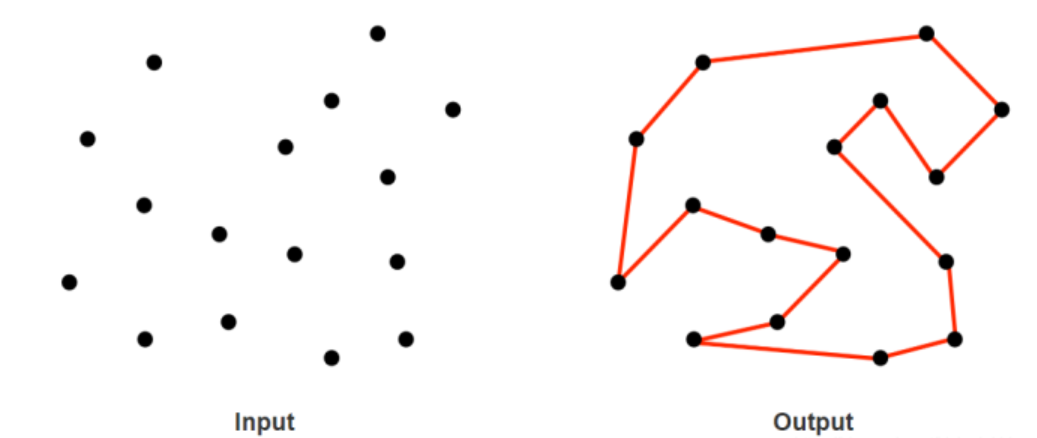
\includegraphics[width=.9\linewidth]{figures/image1.png}
\end{figure}


\subsection{模型求解}
\par 对于这样一个旅行商问题,我们将上述的约束条件编写成python代码,利用贪心算法进行求解。

我们首先处理所有需要配送的书籍订单,将其与位置绑定生成一个字典。接着使用TSP旅行商问题的求解代码进行计算。



\begin{figure}[!htbp]
    \centering
    \begin{minipage}[b]{\linewidth}
        \centering
        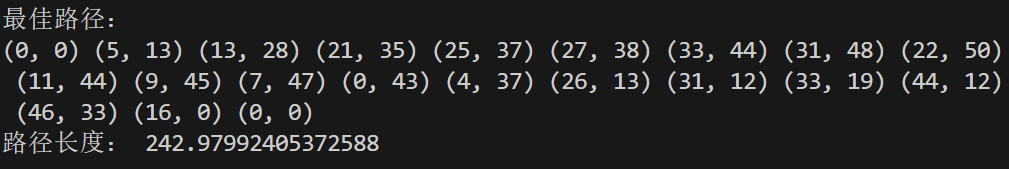
\includegraphics[width=1\textwidth]{figures/result0.1.png}
        \caption{生成的TSP最佳路径}
    \end{minipage}
\end{figure}
\par 绘制出其路径如下图所示
    \begin{figure}[!htbp]
        \centering
        \begin{minipage}[b]{0.85\linewidth}
            \centering
            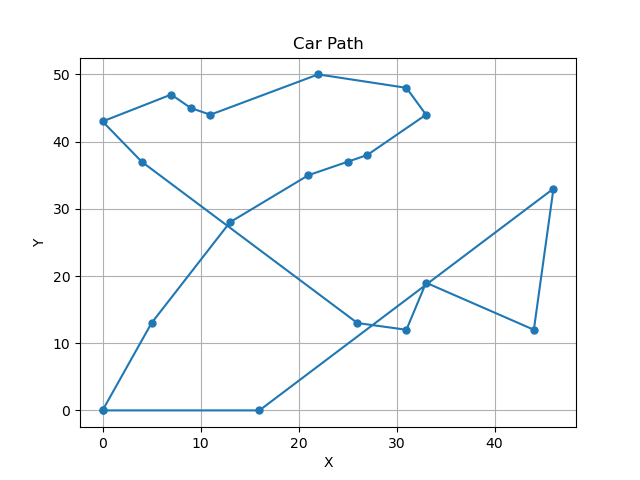
\includegraphics[width=1\textwidth]{figures/result0.2.png}
            \caption{可视化TSP最佳路径}
        \end{minipage}
    \end{figure}
%%%%%%%%%%%%%%%%%%%%%%%%%%%%%%%%%%%%%%%%%%%%%%%%%%%%%%%%%%%%% 

\clearpage
\section{问题二的模型的建立和求解}
\subsection{模型建立}
\par 目标函数 
\begin{equation}
    Z=\operatorname*{min}\sum_{i=0}^{N}\sum_{j=0,j\neq i}^{N}\sum_{k=1}^{M}x_{ijk}\cdot d_{ij}\\
\end{equation}
\par 约束第$k$辆运输小车给书架的配送量不能超过书架的需求量,且只有在运输小车给顾客进行配送时$y_{ik}$ 才有意义
\begin{equation}
   0\leq y_{ik}\leq q_{i}, i\in N, k\in C    
\end{equation}
\par 至少有一辆运输小车为书架进行配送服务
\begin{equation}
    \sum_{i=0}^{N}\sum_{k=1}^{M}x_{ijk}\geq1, j\in N
\end{equation}
\par 到达某点的车辆数应该等于离开该点的车辆数——不会停止不动
\begin{equation}
    \sum_{i=0}^{N}x_{ipk}-\sum_{j=0}^{N}x_{pjk}=0, p\in N, k\in C
\end{equation}
\par 所有书架的取书任务必须全部被完成;
\begin{equation}
   \sum_{k=1}^{M}y_{ik}=q_{i}, i\in N 
\end{equation}
\par 运输小车容量约束,即运输小车的容量必须大于等于运输小车在运输途中为顾客配送的总数量;
\begin{equation}
    \sum_{i=1}^{N}y_{ik}\leq Q, k\in C,0<q_{i}<Q, i\in N
\end{equation}
\par 消除支路限制条件
\begin{equation}
    \sum_{i=0}^{N}\sum_{j=0,j\neq i}^{N}x_{ijk}\leq|s|-1, 2\leq|s|\leq n-1
\end{equation}

\subsection{模型求解}
\par 对于这样一个SDVRP问题,我们将上述的约束条件编写成python代码进行求解

\par \quad ~~~~\textbf{Step1:预处理:} 
我们先对数据进行预处理,生成要图书馆书籍列表,生成书架列表,并且随机选出500本书生成借书列表。
同时我们生成一层图书馆的地图


\begin{figure}[htbp]
    \centering
    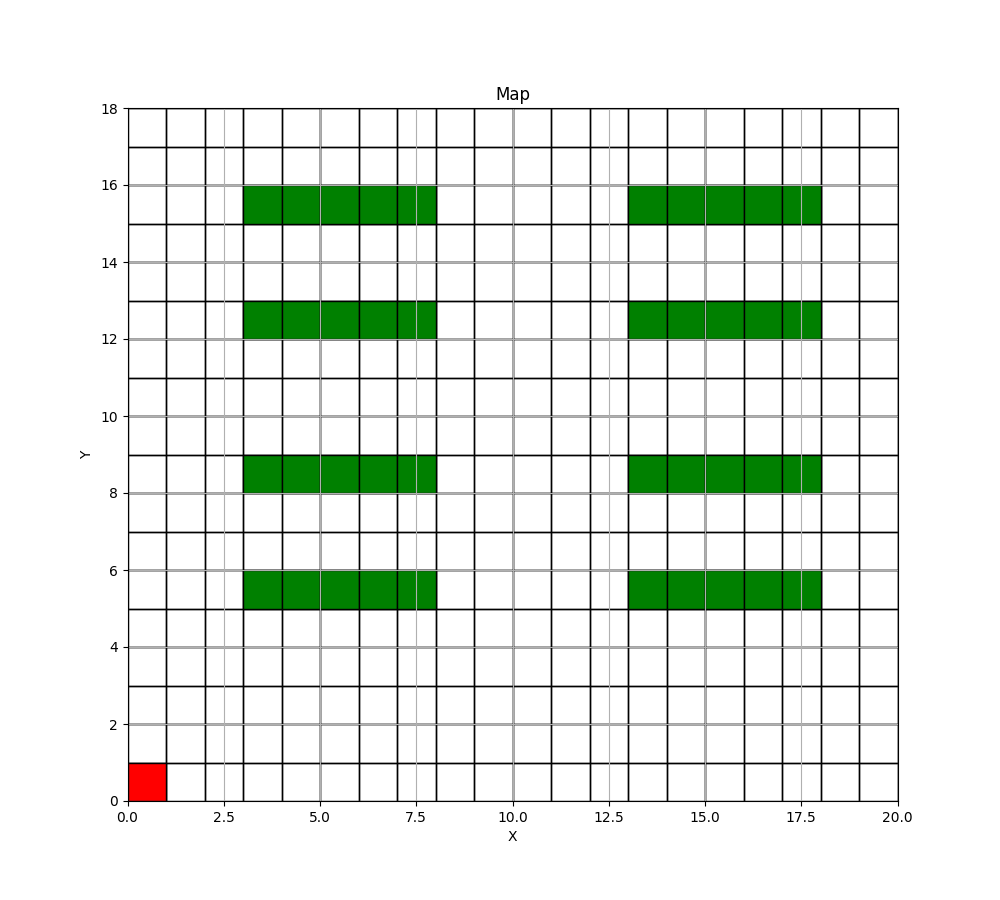
\includegraphics[width=0.5\linewidth]{figures/result1.1.png}
    \caption{libaray map}
\end{figure}

\par \quad ~~~~\textbf{Step2:求解过程} 
\par \textbf{思路1:贪婪算法}
\par 贪婪算法实现:
我们先对建立的数学模型采用贪婪算法,建立SDVRP模型进行求解,求解得到最佳路线和最佳距离
\par 为了更好的阐释贪婪算法求解 SDVRP 问题的步骤,使用伪代码说明算法流程
\begin{breakablealgorithm}
    \caption{贪婪算法求解最优路径}
    \begin{algorithmic}[1]

        \Function {generate\_initial\_solution}{}
            \State 初始化解决方案列表和剩余需求
            \While{剩余需求大于0}
                \State 初始化路线,从原点开始
                \State 初始化剩余容量为车辆容量
                \While{剩余容量大于0且剩余需求大于0}
                    \State 找到可访问的书架并随机访问一个书架
                    \If{剩余容量大于等于书架需求}
                        \State 将书架添加到路线中
                        \State 更新剩余容量和需求
                    \Else
                        \State 将书架添加到路线中
                        \State 更新书架需求和剩余容量为0
                    \EndIf
                \EndWhile
                \State 将路线添加到解决方案中
            \EndWhile
            \State 返回解决方案
        \EndFunction

        \State

        \Function {solve}{$max\_iterations$}
            \State 生成初始解决方案,设置初始解为最佳解
            \State 计算初始解决方案的总距离
            \For{最大迭代次数}
                \State 生成新解并评估其总距离
                \If{新解的总距离小于当前最佳解}
                    \State 更新最佳解和最佳距离
                \EndIf
                \State 记录当前最佳距离到距离历史记录
            \EndFor
            \State 根据路径长度将最佳解分配给小车
            \State 返回最佳解和最佳距离
        \EndFunction   
    \end{algorithmic}
\end{breakablealgorithm}

\par 结果如下图所示,我们可以看出其收敛速度很快,最终找到了总路径较为优秀的解
    \begin{figure}[!htbp]
        \centering
        \begin{minipage}[b]{0.8\linewidth}
            \centering
            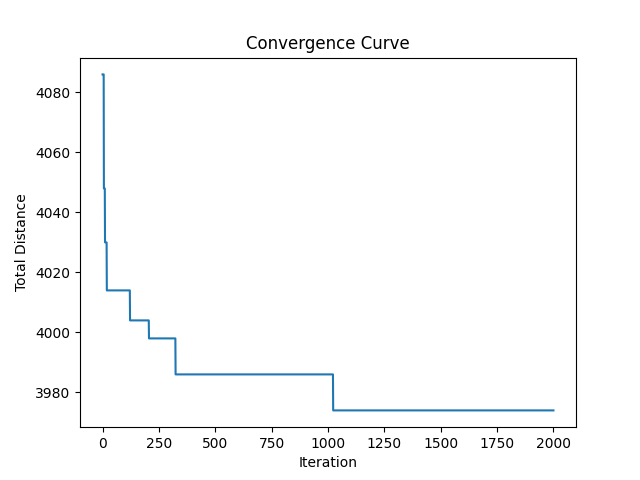
\includegraphics[width=1\textwidth]{figures/result1.2.png}
            \caption{convergence curve}
        \end{minipage}
    \end{figure}

\newpage 

\par \textbf{思路2:蚁群算法}

对于这样一个SDVRP问题,我们采用aco蚁群算法来求解该问题
\par 蚁群算法求解 SDVRP 问题的步骤,同样使用伪代码说明算法流程
\begin{breakablealgorithm}
    \caption{蚁群算法求解最优路径}
    \begin{algorithmic}[1]
        \Function {ACO}{}
        \State 初始化蚁群
        \State 初始化信息素矩阵
        \For{$iteration = 1$ \textbf{to} $num\_iterations$}
            \For{每只蚂蚁}
                \State 构建解决方案
                \State 计算路径长度
                \If {当前路径长度 $<$ 最佳路径长度}
                    \State 更新最佳路径和最佳路径长度
                \EndIf
            \EndFor
            \State 更新信息素
            \State 打印当前迭代的最佳路径长度
        \EndFor
        \State \textbf{return} 最佳路径, 最佳路径长度
        \EndFunction
        
        \Function{ConstructSolution}{蚂蚁}
            \For{每辆车}
                \While{存在未访问的书架}
                    \State 选择下一个要访问的书架
                    \State 更新小车路径和书架的访问状态
                \EndWhile
                \State 小车返回起点
            \EndFor
        \EndFunction
        
        \Function{UpdatePheromones}{蚁群}
            \State 依据路径长度更新信息素
        \EndFunction
    \end{algorithmic}
\end{breakablealgorithm}

\par 结果如下图所示,我们可以看出相对于贪婪算法其收敛速度更快,需要的迭代次数更少,并且能够得出更为优秀的最优路径
\newpage
\begin{figure}[!htbp]
    \centering
    \begin{minipage}[b]{0.7\linewidth}
        \centering
        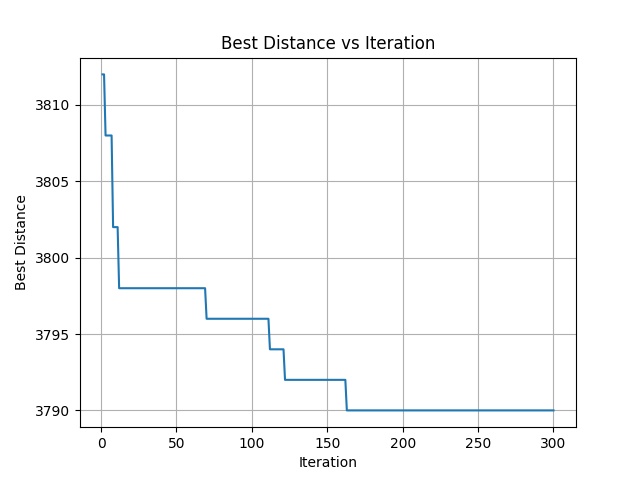
\includegraphics[width=1\textwidth]{figures/aco_convergence.png}
        \caption{aco convergence}
    \end{minipage}
\end{figure}

\par 下图显示求得的小车总的最优路径

\begin{figure}[!htbp]
    \centering
    \begin{minipage}[b]{0.7\linewidth}
        \centering
        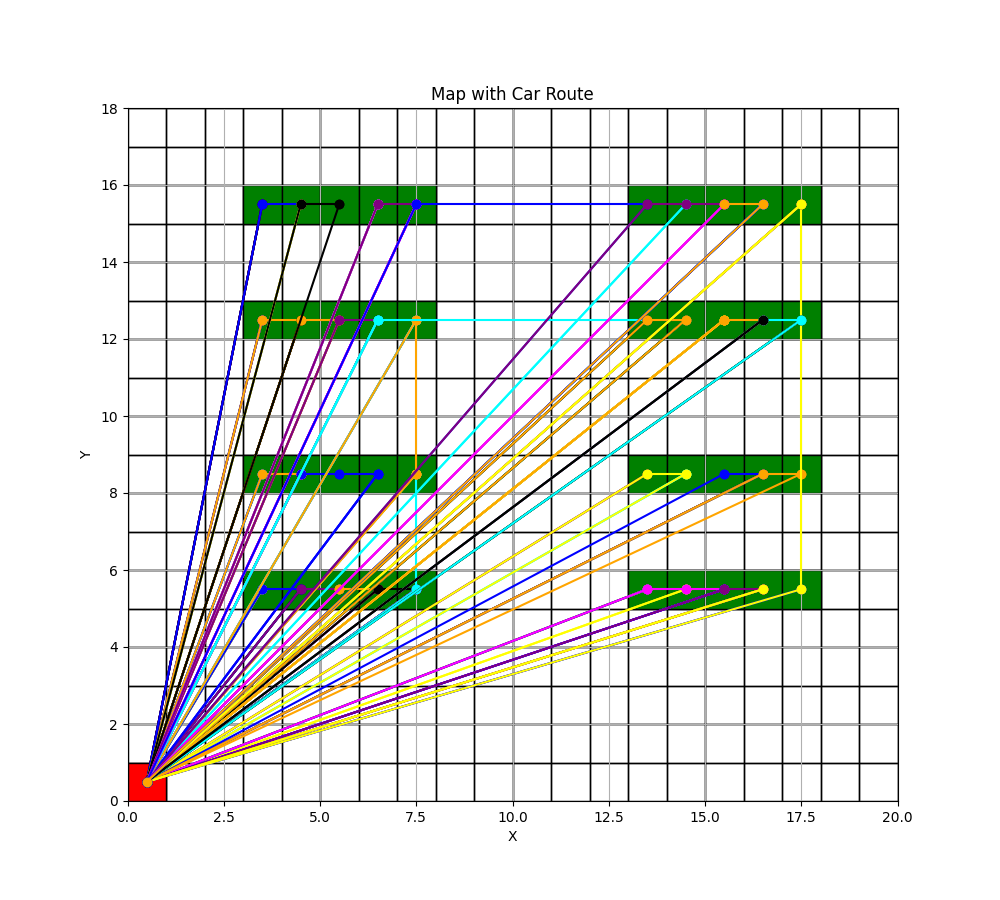
\includegraphics[width=1\textwidth]{figures/map_with_route.png}
        \caption{vehicle with route}
    \end{minipage}
\end{figure}

\par 在寻找到最佳路线后,我们尝试将路线分配给四个运输小车,采用贪心算法,使每辆小车的运输任务趋于一致。最后求得每辆运输小车各自的运输任务路径。
\newpage
\begin{breakablealgorithm}
    \caption{贪心算法分配小车任务}
    \begin{algorithmic}[1]
        \Function {split\_routes}{$routes, num\_vehicles$}
            \State 计算每条路线的总距离
            \State 将路线按距离从大到小排序
            \State 初始化车辆路线列表和车辆负载列表
            \For{每条排序后的路线}
                \State 找到负载最小的小车
                \State 将路线分配给该小车
                \State 更新小车负载
            \EndFor
            \State 返回小车路线列表
        \EndFunction
    \end{algorithmic}
\end{breakablealgorithm}

\par 下图显示四辆小车分别的运输路径。
    \begin{figure}[!htbp]
        \centering
        \begin{minipage}[b]{0.75\linewidth}
            \centering
            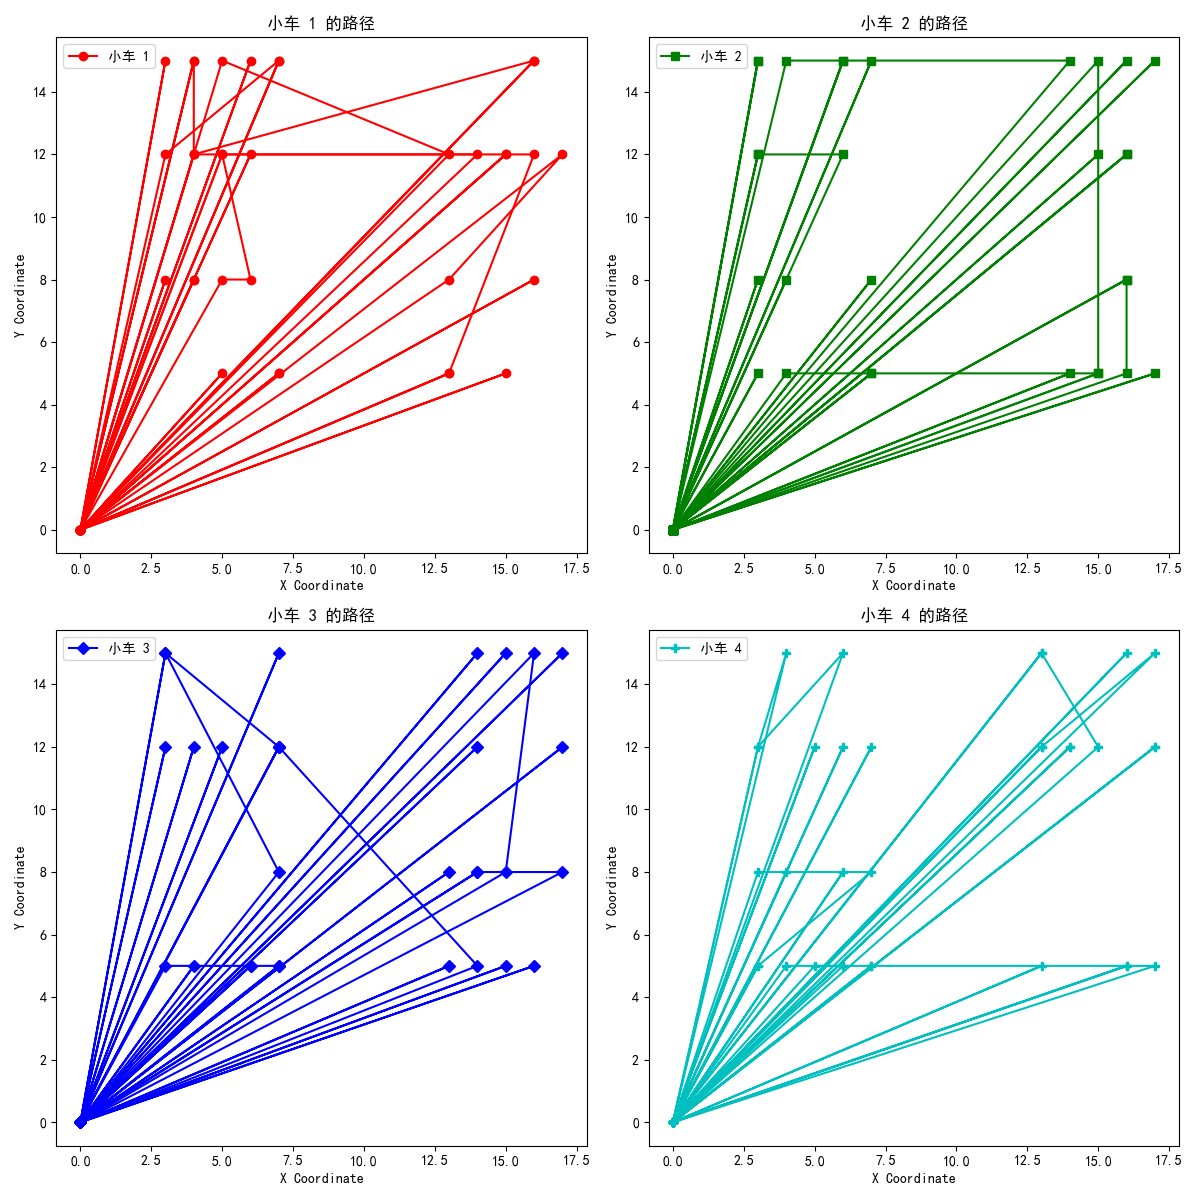
\includegraphics[width=1\textwidth]{figures/result1.3.png}
            \caption{vehicle route}
        \end{minipage}
    \end{figure}

    
\clearpage
\section{问题三的模型的建立和求解}
\subsection{模型建立}
\par 目标函数
\begin{equation}
   min \sum_{i\in I }^{} (d_{iqm}+d_{imq}+d_{imr})
\end{equation}
\par \textbf{1.托盘内书本数量与预约订单匹配约束}
\par 虑托盘i在拣选工位应被挑选走的第h种书的数量小于第i个托盘里拥有第h种书得数量
\begin{equation}
    0 \le k_{ih} \le O_{ih}, \forall i \in I,h \in H
\end{equation}
\par 考虑若托盘 $i$ 被挑选出前往书本拣选节点,则从托盘$i$ 中挑选出来的书本数量总和应大于 0
\begin{equation}
    \sum _ {h \in H}^ {} k_{ih} +M(1-  x_ {i}  )>0,  \forall i \in I	
\end{equation}
\par 考虑若托盘 $i$ 没有被挑选出前往书本拣选节点,则从托盘$i$ 中挑选出来的书本数量总和应等于 0
\begin{equation}
    \sum_{h \in H}{}k_{ih}- \sum_{h \in H}{}O_{ih}×x_i\leqslant 0, \forall i\in I	
\end{equation}
\par 限制从所有托盘中取出的第h种书本的数量应等于预约中需求的数量
\begin{equation}
    \sum _ {i\in I}^ {}  k_ {ih} =  C_ {h} ,  \forall  i  \in I,h  \in  H	
\end{equation}
\par 托盘中的书籍全部被挑选走:当且仅当托盘i中的书籍被完全挑选走时,$y_i$才等于 1。
\begin{equation}
    1 \leqslant y_i+M×\sum_{h \in H} (O_{ih} - k_{ih} )	
\end{equation}
\par 如果没有被挑选完,$y_i$等于0
\begin{equation}
    y_i × \sum_{h \in H}O_{ih} \leqslant\sum_{h \in H}k_{ih}	
\end{equation}
\par \textbf{2.托盘与书籍挑选节点的匹配}
\par 考虑托盘 $i$ 至多前往一个拣选工作台
\begin{equation}
    \sum _ {m \in M}^ {} p_ {im}   \leqslant  1, \forall  i  \in I	
\end{equation}
\par 考虑若托盘 i 前往拣选工作台,限制其一定会被指派前往一个拣选工作台
\begin{equation}
    \sum _ {m\in M}^ {}  p_ {im}  -  x_ {i}  =0,  \forall  i  \in  I	
\end{equation}
\par 考虑若托盘i从储位 q 被挑选出前往拣选工作台m,则托盘i从储位q至拣选工作台 m 的行走路线长度$d_{iqm}$应大于从储位q至拣选工作台 *m* 的最短路径$D_{qm}$
\begin{equation}
    d_ {iqm}  +M(3-  x_ {i}  -  p_ {im}  -  J_ {iq}  )  \geqslant   D_ {qm}  ,  \forall  i  \in  I,m  \in  M,q  \in  Q	
\end{equation}
\par 考虑若托盘i从储位q没有被挑选出前往拣选工作台m,则托盘i从储位q至拣选工作台m的行走路线长度$d_{iqm}$应等于0
\begin{equation}
    d_ {iqm}  -M x_ {i}  \leqslant  0,  \forall  i  \in I,m  \in M,q \in  Q   
\end{equation}
\par \textbf{3.如果托盘还有书籍,则需要放到空储位节点}
\par 考虑若托盘i没有被挑选出前往拣选工位,则托盘i中必有书籍存在
\begin{equation}
    x_ {i}  -  y_ {i}  \geqslant 0,  \forall  i  \in I   
\end{equation}
\par 考虑托盘i在被拣选完后,托盘可能为空也可能非空,至多前往一个储位
\begin{equation}
    \sum _ {q\in Q}^ {}   g_ {iq}   \leqslant  1,  \forall  i  \in I   
\end{equation}
\par  考虑如果托盘i中的书籍未被全部挑选出来,即托盘i中被拣选之后还有剩余书籍,则为其分配一个储位
\begin{equation}
    y_ {i}  +  \sum _ {q \in Q}^ {}   g_ {iq}   = x_i, \forall  i \in I   
\end{equation}
\par 考虑若托盘i没有被挑选出前往拣选工作台,则不需要为其分配储位
\begin{equation}
    x_ {i}  -  \sum _ {q\in Q}^ {}  g_ {iq}   \geqslant  0,  \forall  i  \in I   
\end{equation}
\par 考虑任意一个托盘被挑选完后只能前往储位或空盘回收位中的一个
\begin{equation}
    \sum _ {q \in Q}^ {}   g_ {iq}  +  \sum _ {r\in R}   f_ {ir}  = x_i,  \forall i \in I   
\end{equation}
\par 考虑托盘i在拣选之后分配的储位仅能为空储位
\begin{equation}
    g_ {iq}  -  z_ {q}   \leqslant  0, \forall  i \in I,q  \in  Q
\end{equation}
\par 约束一个储位只能有一个托盘
\begin{equation}
    \sum_{i \in I}g_{iq} \leqslant 1,\forall q \in Q  
\end{equation}

\par 考虑托盘i没有被挑选出前往拣选工作台,或托盘中的书籍被挑选空,则托盘从拣选工作台m 至空储位q的行走路线长度应为 0
\begin{equation}
   d_ {imq} -M(x_ {i}  -  y_ {i} )  \leqslant 0,  \forall  i  \in I,m  \in  M,q  \in Q
\end{equation}
\par 考虑托盘i被挑选出前往拣选工作台并且前往拣选工作台 m,挑选完成后托盘非空,则托盘从拣选工作台至空储位q的行走路线长度$d_{imq}$应大于从拣选工作台m至储位q的最短路径$D_{mq}$ 
\begin{equation}
    d_ {imq}  +M(4-  x_ {i}  +  y_ {i}  -  p_ {im}  -  g_ {iq}  -  z_ {q}  )  \geqslant  D_ {mq}  , \forall  i  \in  I,m  \in M,q  \in  Q   
\end{equation}
\par 若托盘i被挑选走,则其所在的储位q是空储位
\begin{equation}
    z_ {q}  +  J_ {iq}  -  x_ {i}  \leqslant  1,  \forall i  \in I,q  \in  Q   
\end{equation}
\par \textbf{4.若托盘无书籍,则考虑托盘与回收节点的匹配}
\par 考虑托盘i中的书籍全部被挑选走,则从托盘i中挑选出来的书籍数量总和应等于托盘i中拥有的书籍数量总和
\begin{equation}
    \sum_{h\in H}{}k_{ih} - \sum_{h \in H}{}O_{ih}+M(1-y_i)  \geqslant 0, \forall i \in I   
\end{equation}
\par 托盘i在被拣选完商品后,至多前往一个空盘回收位
\begin{equation}
    \sum_{r \in R}{}f_{ir} \le 1,\forall i \in I   
\end{equation}
\par 考虑如果托盘i被挑选后没有书籍,则分配一个回收处,如果挑选后还有书籍,则不分配回收处
\begin{equation}
    \sum_{r \in R}{}f_{ir} = y_i,\forall i \in I  
\end{equation}
\par 托盘i没有被挑选出前往拣选工作台,则不需要为其分配空盘回收位
\begin{equation}
    x_ {i}  -  \sum _ {r\in R}^ {}  f_ {ir}   \geqslant  0,  \forall  i  \in I   
\end{equation}
\par 考虑托盘i被挑选出前往拣选工作台并且前往拣选工作台 m,挑选完成后托盘非空,则托盘从拣选工作台至空储位q的行走路线长度$d_{imr}$应大于从拣选工作台m至储位q的最短路径$D_{mr}$ 
\begin{equation}
   d_ {imr}  +M(4-  x_ {i}  -  y_ {i}  -  p_ {im}  -  f_ {ir} )  \geqslant  D_ {mr}  , \forall  i  \in  I,m  \in M,q  \in  Q
\end{equation}

\newpage

\subsection{模型求解}
\par \textbf{思路1:pulp求解器}
\par 对于这样一个MLP问题,我们将上面的约束条件直接编写python代码进行求解,利用Python的PULP库即可。
\par 但是对于大数据来说,求解为了验证其正确性,我们首先采用了小数据进行求解,来验证其正确性。
\par 对于地图的颜色标注,我们有以下规定:
\par \quad \quad \quad \textbf{GREEN:}货架,用来存放装有书的托盘
\par \quad \quad \quad \textbf{YELLOW:}托盘回收处
\par \quad \quad \quad \textbf{BLACK:}障碍物,智能机器人不能通行
\par \quad \quad \quad \textbf{RED:}书籍挑拣点\newline



\par\textbf{ Example1:}

小地图,预定书籍=当前处理书籍
\par 我们指定有5个托盘,分别存储在下图2的货架1,3,5,7,9中。每个托盘分别存储着3本书,该例中,当前处理书籍是托盘内的所有书,因此所有托盘都被指派且将到达回收处。根据solve1.py的求解结果(见图一),由diqm,dimq,dimr的值可以画出如下托盘路径,与期望的最短路径相同。

\begin{figure}[!htbp]
    \centering
    % \begin{minipage}[b]{0.8\linewidth}
        \begin{minipage}[b]{0.4\linewidth}
            \centering
            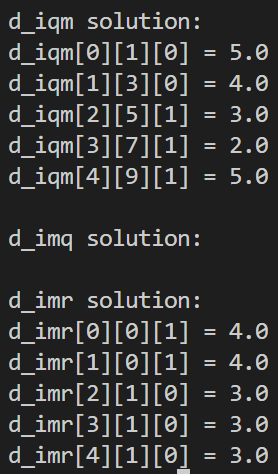
\includegraphics[width=0.6\textwidth]{figures/result2.1.png}
            \caption{运行结果}
        \end{minipage}%
        \begin{minipage}[b]{0.58\linewidth}
            \centering
            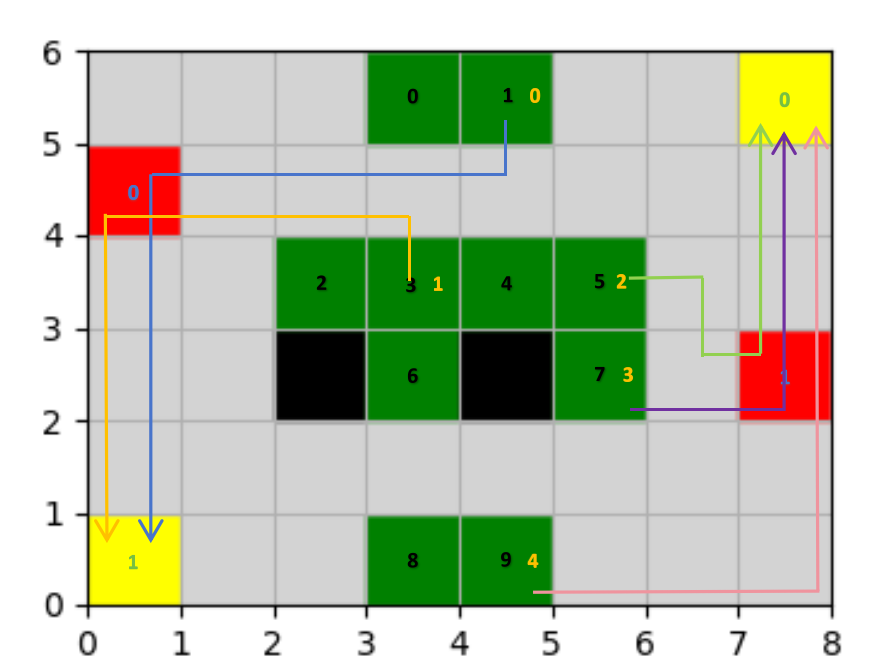
\includegraphics[width=1\textwidth]{figures/2.1.png}
            \caption{路径图示}
        \end{minipage}
    % \end{minipage}
\end{figure}

\par \textbf{Example2:} 小地图,预定书籍>当前处理书籍
\par 类似Example1,不同点在于,当前处理书籍设置成部分库存。根据solve2.py的求解结果,由diqm,dimq,dimr的值可以画出如下托盘路径,与期望的最短路径相同。  
\par 下面详细说明Example1与Example2的区别以及测试目的:
\par Example2在要处理的书籍中去除了托盘2的书籍18,和托盘3的书籍4。直观上初步认为托盘2和托盘3将回到储位。但结果显示托盘0回到储位2,托盘2去了回收处0,托盘3回到了储位7。这是由于托盘0内有书籍18和4,而托盘0->挑拣处0->储位2+托盘2->挑拣处1->回收处0的值小于托盘0->挑拣处0->回收处1+托盘2->挑拣处1->储位3。该例巧妙地说明了我们的程序确实是向着总路程最小的方向走。


\par 

\begin{figure}[!htbp]
    \centering
    % \begin{minipage}[b]{0.8\linewidth}
        \begin{minipage}[b]{0.4\linewidth}
            \centering
            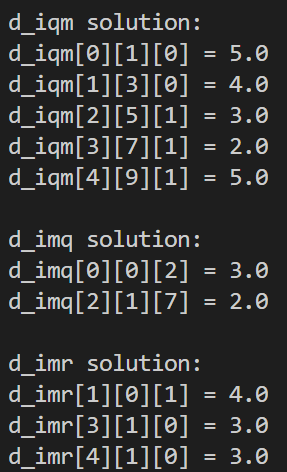
\includegraphics[width=0.6\textwidth]{figures/result2.2.png}
            \caption{运行结果}
        \end{minipage}%
        \begin{minipage}[b]{0.58\linewidth}
            \centering
            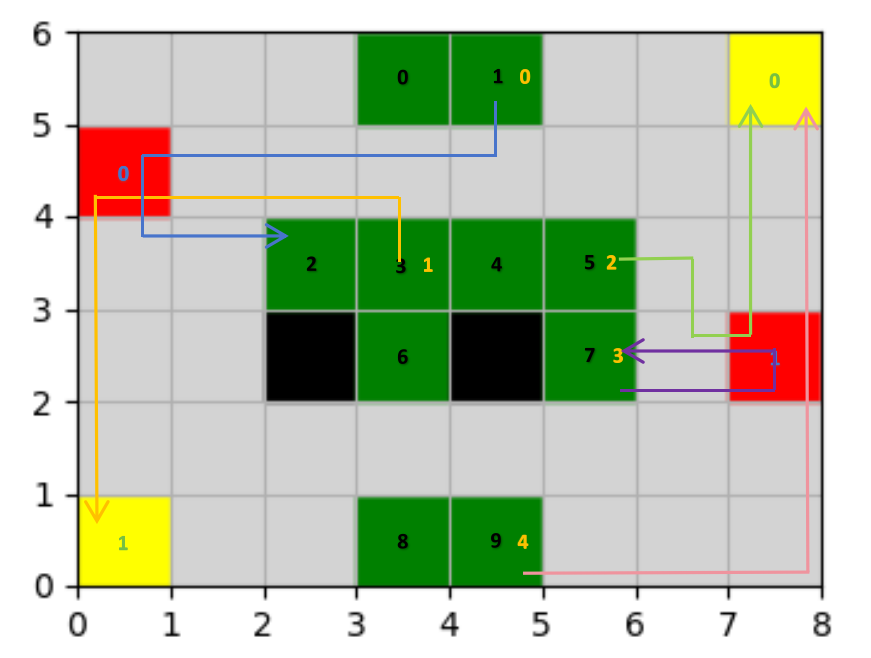
\includegraphics[width=1\textwidth]{figures/2.2.png}
            \caption{路径图示}
        \end{minipage}
    % \end{minipage}
\end{figure}

\par 对于大数据来说,原来的小地图并不能满足,因此我们构建新地图,如下图所示

\begin{figure}[!htbp]
    \centering
    \begin{minipage}[b]{\textwidth}
        \centering
        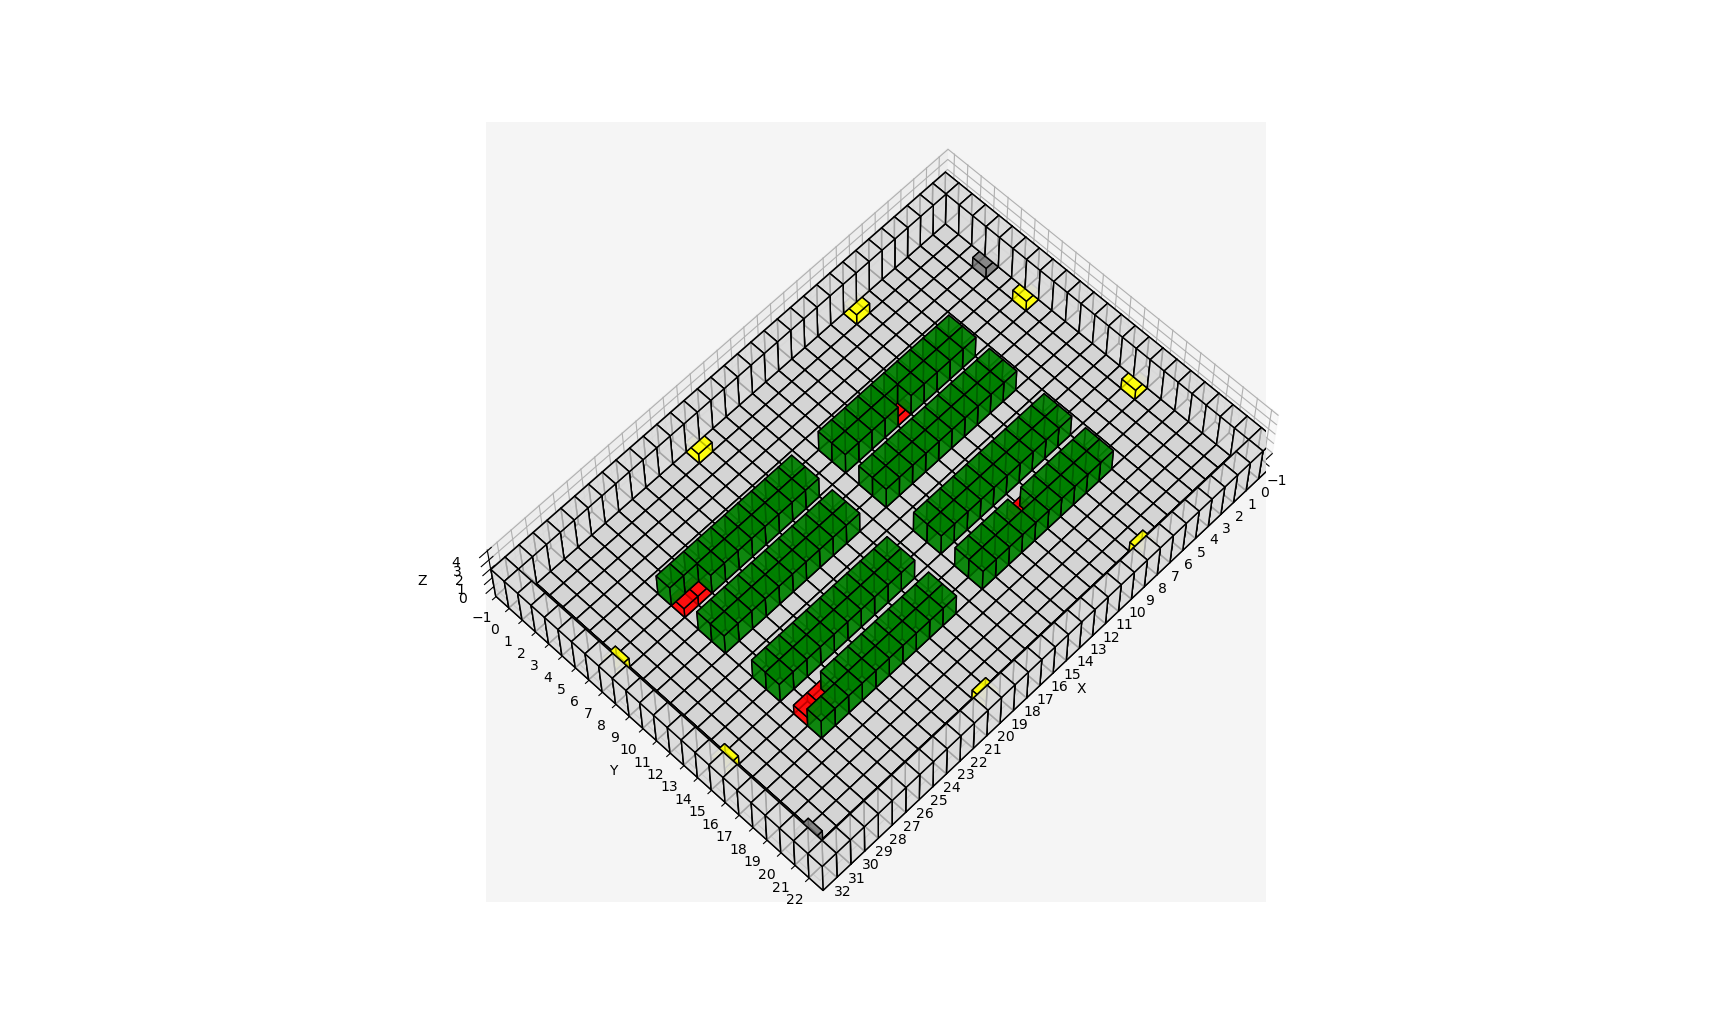
\includegraphics[width=1\textwidth]{figures/map2.png}
        \caption{大数据地图}
    \end{minipage}
\end{figure}

\newpage
\par \textbf{Example3:} 大地图,预定书籍=当前处理书籍
\par 我们指定有20个托盘,存储在下图的154个货架中。每个托盘分别存储不同数量的书,该例中,当前处理书籍是托盘内的所有书,因此所有托盘都被指派且将到达回收处。根据solve3.py的求解结果,该例结果为,所有托盘被运到挑拣处并到达回收处的总路程为370


\begin{figure}[!htbp]
    \centering
    \begin{minipage}[b]{\linewidth}
        \centering
        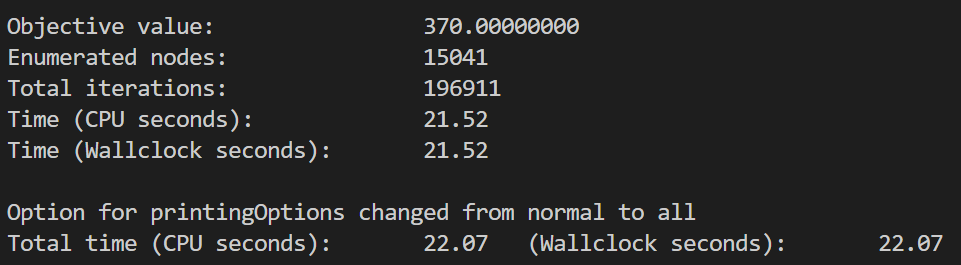
\includegraphics[width=0.9\textwidth]{figures/result2.3.png}
        \caption{最短路径}
    \end{minipage}
\end{figure}

\par 三步的距离如下图所示
    
\begin{figure}[!htbp]
    \centering
    \begin{minipage}[b]{\linewidth}
        \centering
        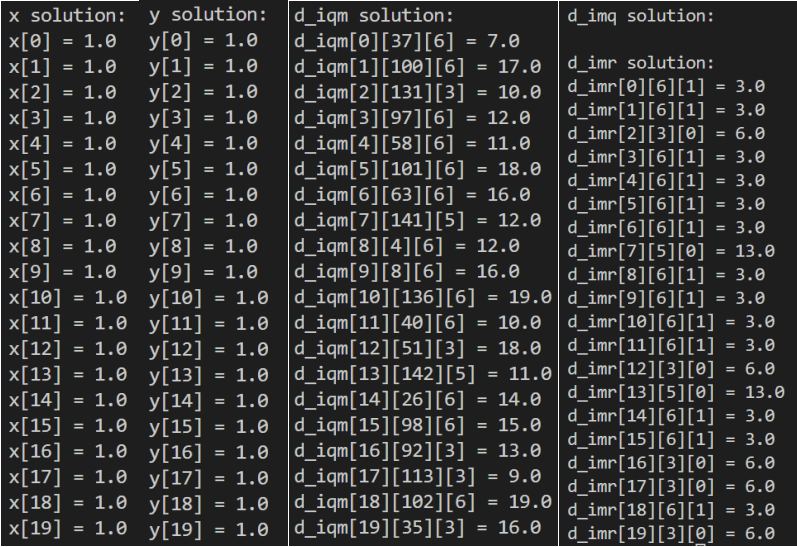
\includegraphics[width=0.9\textwidth]{figures/result2.4.png}
        \caption{各步距离}
    \end{minipage}
\end{figure}

\newpage
\par \textbf{Example4:} 大地图,预定书籍>当前处理书籍
\par 由于大数据量带来的地图过大带来的维度过高,对于MLP的求解器负荷过高,故设置较少的托盘,现在设置12个托盘,运行结果如下图所示。

\begin{figure}[!htbp]
    \centering
    \begin{minipage}[b]{\linewidth}
        \centering
        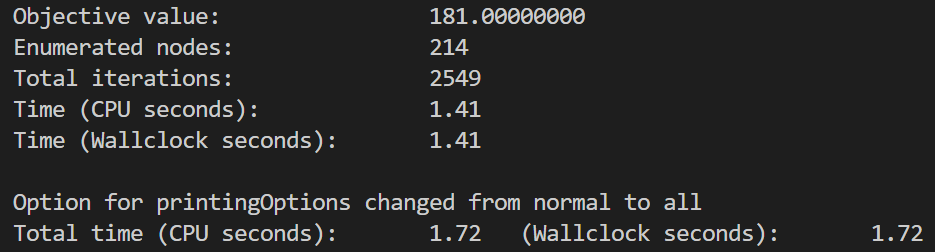
\includegraphics[width=0.9\textwidth]{figures/result2.5.png}
        \caption{最短路径}
    \end{minipage}
\end{figure}

\par 根据 solve3.py 的求解结果,该例结果为,所有托盘被运到挑拣处并到达回收处的总路程为 181

\par 三步的距离如下图所示


\begin{figure}[!htbp]
    \centering
    \begin{minipage}[b]{0.55\linewidth}
        \centering
        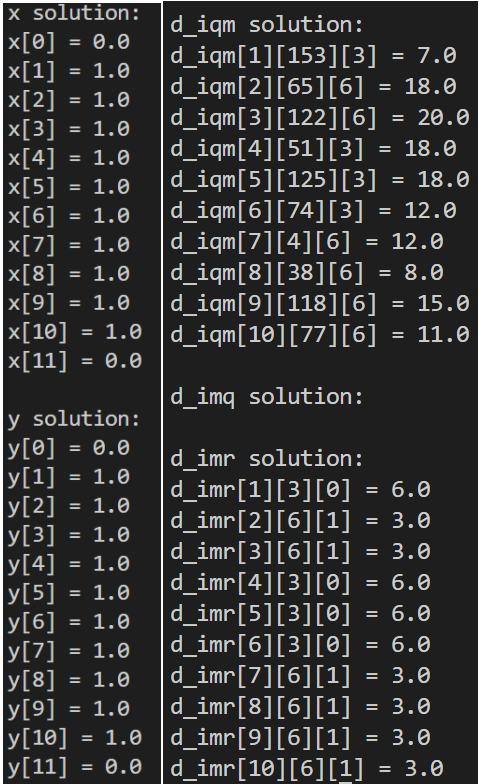
\includegraphics[width=0.9\textwidth]{figures/result2.6.png}
        \caption{各步距离}
    \end{minipage}%
\end{figure}

\newpage
\par \textbf{思路2:遗传算法}
\par 对于这样一个MLP问题,我们用遗传算法与deap库来求解该问题
\par \textbf{Example1:} 小地图,预定书籍=当前处理书籍
\par 运行结果为最短路程:97,如图\ref{d}所示
    \begin{figure}[!htbp]
        \centering
        \begin{minipage}[b]{0.3\linewidth}
            \centering
            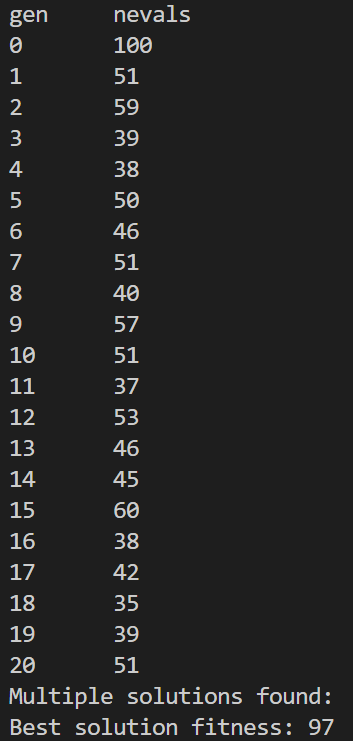
\includegraphics[width=0.6\textwidth]{figures/3.1.png}
            \caption{迭代结果}
            \label{d}
        \end{minipage}%
        \begin{minipage}[b]{0.7\linewidth}
            \centering
            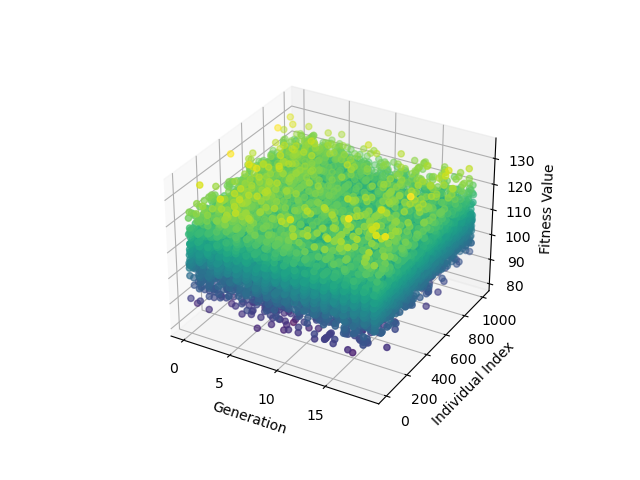
\includegraphics[width=1\textwidth]{figures/3.1.1.png}
            \caption{图形可视化}
        \end{minipage}%
    \end{figure}
\par \textbf{Example2:} 小地图,预定书籍>当前处理书籍
\par 运行结果为最短路程:102,如图\ref{dd}所示
    \begin{figure}[!htbp]
        \centering
        \begin{minipage}[b]{0.3\linewidth}
            \centering
            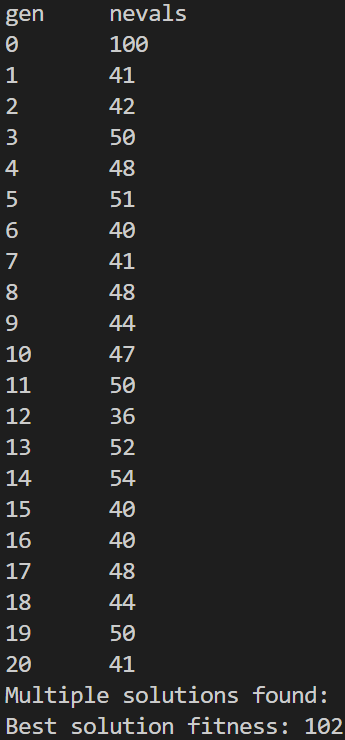
\includegraphics[width=0.6\textwidth]{figures/3.2.png}
            \caption{迭代结果}
            \label{dd}
        \end{minipage}%
        \begin{minipage}[b]{0.7\linewidth}
            \centering
            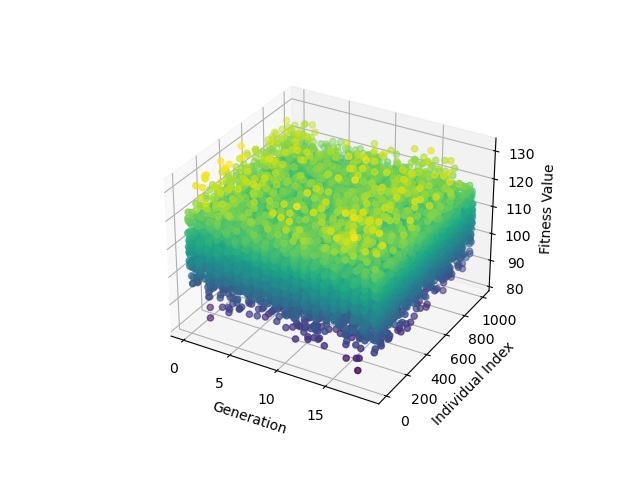
\includegraphics[width=1\textwidth]{figures/3.2.1.png}
            \caption{图形可视化}
        \end{minipage}%
    \end{figure}



% \begin{figure}[!htbp]
%         \centering
%         \subcaptionbox{图形可视化}[0.45\textwidth][c]{
%             \centering
%             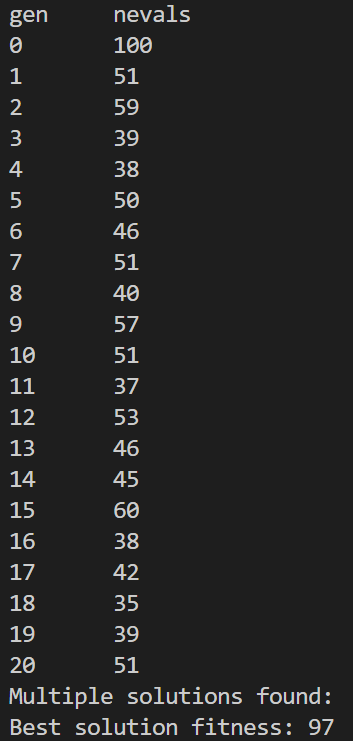
\includegraphics[width=0.6\width]{figures/3.1.png}
%             \label{d}
%         }%
%         \hspace*{0.1cm}
%         \subcaptionbox{四个子图2}[0.45\textwidth][c]{
%             \centering
%             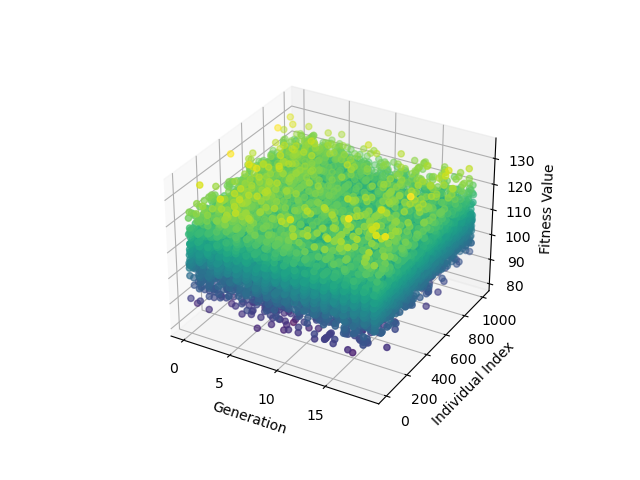
\includegraphics[width=1\linewidth]{figures/3.1.1.png}
%         }\\% % 换行
%         \subcaptionbox{迭代结果}[0.45\textwidth][c]{
%             \centering
%             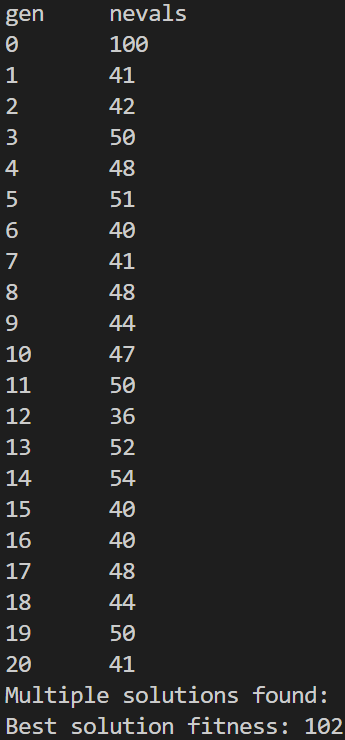
\includegraphics[width=0.6\linewidth]{figures/3.2.png}
%             \label{dd}
%         }%
%         \hspace*{0.1cm}
%         \subcaptionbox{图形可视化}[0.45\textwidth][c]{
%             \centering
%             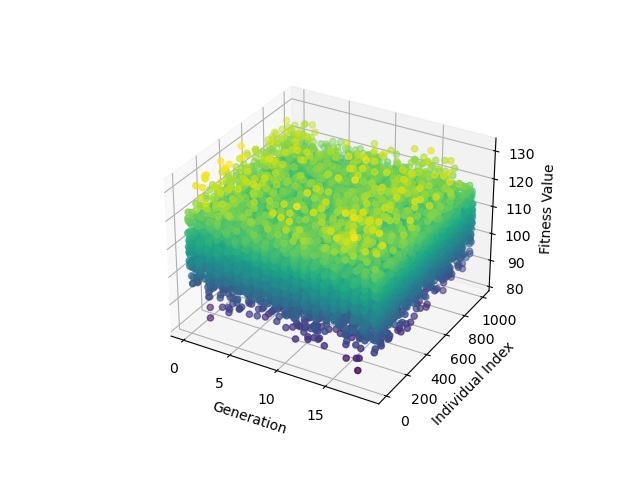
\includegraphics[width=1\linewidth]{figures/3.2.1.png}
%         }%
%     \end{figure}
\par \textbf{Example3:} 大地图,预定书籍=当前处理书籍
\par 运行结果为最短路程:24596
    \begin{figure}[!htbp]
        \centering
        \begin{minipage}[b]{0.4\linewidth}
            \centering
            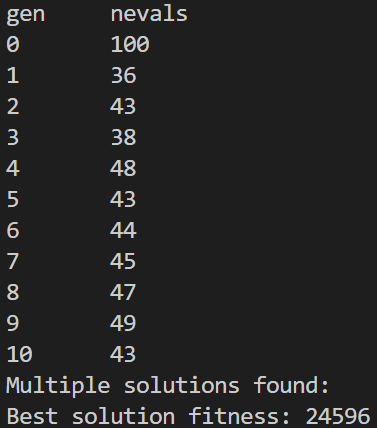
\includegraphics[width=0.9\textwidth]{figures/3.3.png}
            \caption{迭代结果}
        \end{minipage}%
        \begin{minipage}[b]{0.53\linewidth}
            \centering
            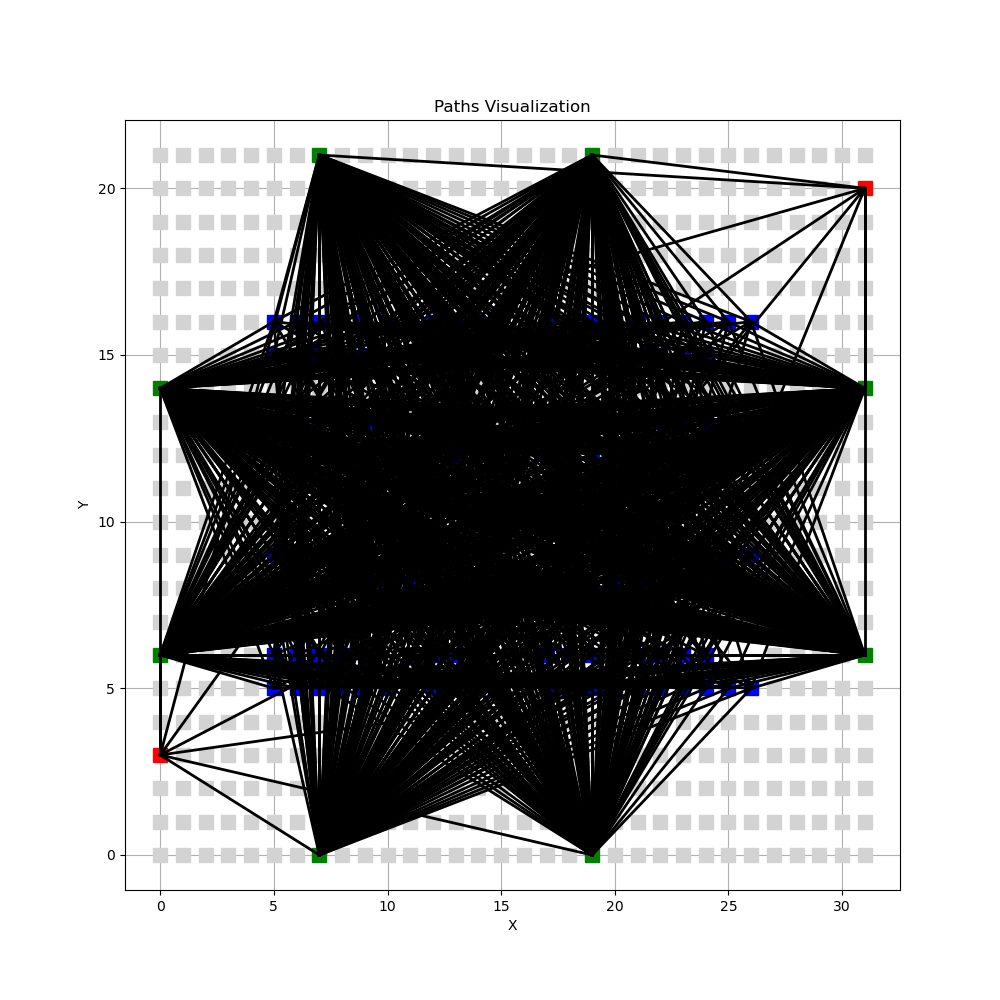
\includegraphics[width=0.9\textwidth]{figures/3.4.png}
            \caption{路径可视化}
        \end{minipage}%
    \end{figure}

\par \textbf{Example4:} 大地图,预定书籍>当前处理书籍
\par 运行结果为最短路程:14715
    \begin{figure}[!htbp]
        \centering
        \begin{minipage}[b]{0.4\linewidth}
            \centering
            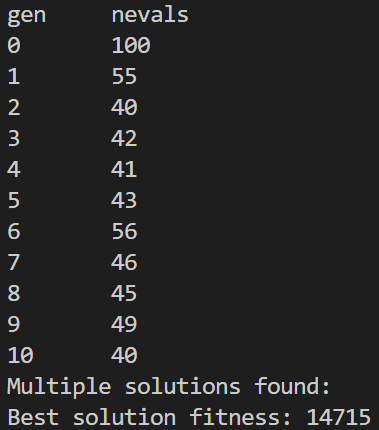
\includegraphics[width=0.9\textwidth]{figures/3.5.png}
            \caption{迭代结果}
        \end{minipage}%
        \begin{minipage}[b]{0.53\linewidth}
            \centering
            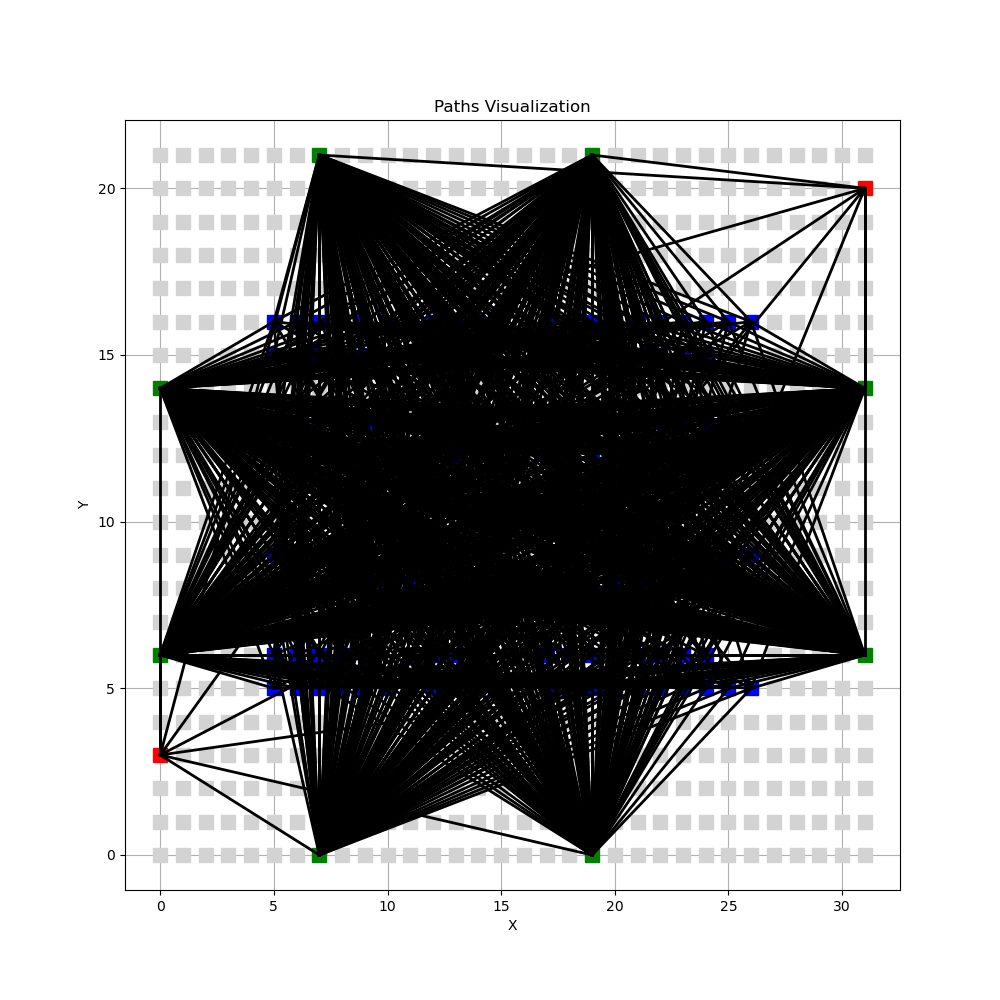
\includegraphics[width=0.9\textwidth]{figures/3.6.png}
            \caption{路径可视化}
        \end{minipage}%
    \end{figure}


%%%%%%%%%%%%%%%%%%%%%%%%%%%%%%%%%%%%%%%%%%%%%%%%%%%%%%%%%%%%%

\clearpage
\section{模型的分析与检验}


\par \textbf{针对问题二}
\par 我们选择对蚁群算法进行灵敏度分析,蚁群算法的参数指标主要是alpha,beta和evaporation\_rates信息素浓度,以下图像是三个指标对结果数据的影响。
\begin{figure}[!htbp]
    \centering
    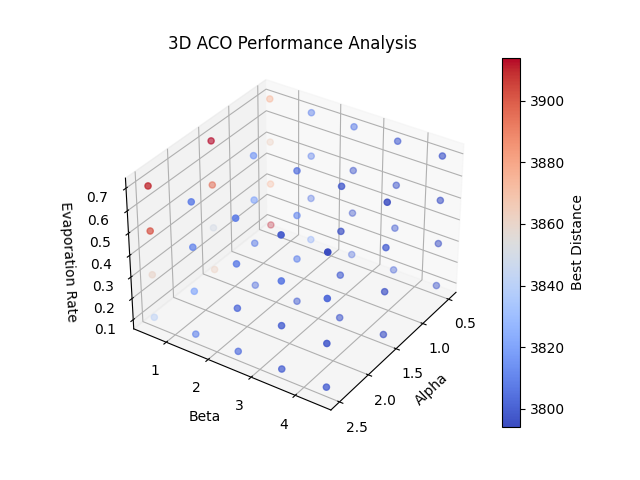
\includegraphics[width=0.8\textwidth]{figures/senstivity2.png}
    \caption{灵敏度分析}
\end{figure}
\par \textbf{1.参数影响的直观观察:}
从图形表示中可以观察到,代表蚁群优化(ACO)算法找到的最佳路径长度或成本的点的颜色随着参数\textit{alpha}、\textit{beta}和\textit{evaporation rate}的变化而变化,这表明这些参数确实影响了算法的最终结果。红色点代表更高的成本,而蓝色点表示更低的成本,显示了在某些参数组合下算法找到了更短的路径。

\par \textbf{2.Alpha的影响:}
\textit{Alpha}参数控制信息素的重要性。从图像上看,当\textit{Alpha}增加时,路径长度的变化似乎不是单调的,这可能意味着存在一个最优的\textit{Alpha}值范围,而不是越大或越小越好。

\par \textbf{3.Beta的影响:}
\textit{Beta}参数控制启发式信息的影响力。图中显示,\textit{Beta}值的变化同样没有表现出明显的单调趋势,这表明启发式信息在平衡信息素影响力时起到关键作用。

\par \textbf{4.Evaporation Rate的影响:}
信息素的蒸发率似乎对算法性能有显著影响。在较低的蒸发率(接近0.1)时,算法找到的路径似乎更优,这可能表明较低的蒸发率有助于保留有价值的路径信息,从而指导搜索过程。

\par \textbf{5.参数间的交互效应:}
图中数据点的分布可能还揭示了参数间的复杂交互关系。例如,在特定的\textit{alpha}和\textit{beta}组合下,某些\textit{evaporation rates}可能更有效,这表明调整单一参数可能不足以显著改善性能,而需要综合考虑多个参数的调整。


\par \textbf{针对问题三·}
\par 对于遗传算法进行误差分析,我们进行了多次运算并对其进行误差分析
\par 对于Example1,其均值、标准差以及最坏最好值如下
    \begin{figure}[!htbp]
        \centering
        \begin{minipage}[b]{0.5\linewidth}
            \centering
            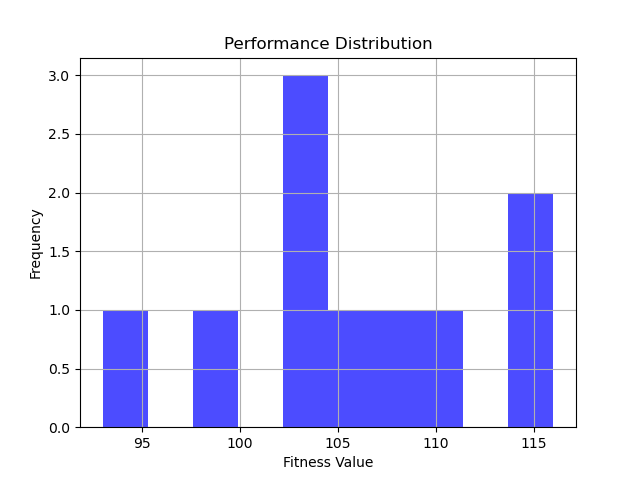
\includegraphics[width=0.9\textwidth]{figures/4.1.png}
            \caption{运行结果}
        \end{minipage}%
        \begin{minipage}[b]{0.48\linewidth}
            \centering
            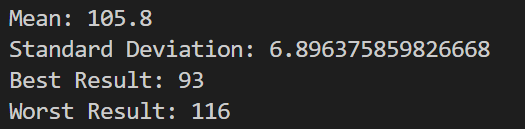
\includegraphics[width=0.9\textwidth]{figures/4.2.png}
            \caption{数学指标}
        \end{minipage}%
    \end{figure}
\par 对于Example2,其均值、标准差以及最坏最好值如下
    \begin{figure}[!htbp]
        \centering
        \begin{minipage}[b]{0.5\linewidth}
            \centering
            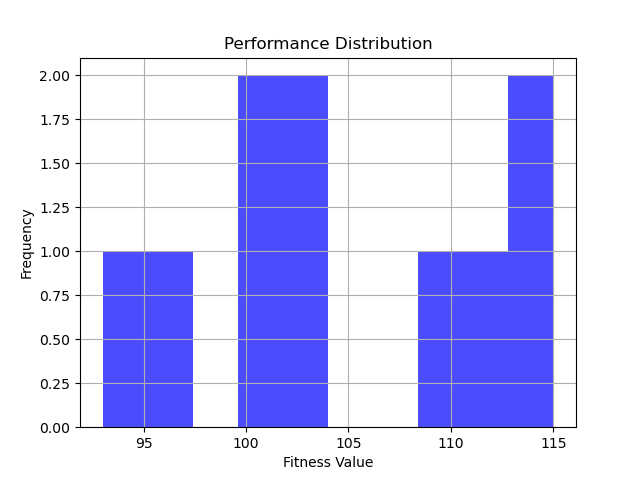
\includegraphics[width=0.9\textwidth]{figures/4.3.png}
            \caption{运行结果}
        \end{minipage}%
        \begin{minipage}[b]{0.48\linewidth}
            \centering
            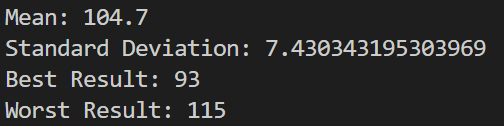
\includegraphics[width=0.9\textwidth]{figures/4.4.png}
            \caption{数学指标}
        \end{minipage}%
    \end{figure}
%%%%%%%%%%%%%%%%%%%%%%%%%%%%%%%%%%%%%%%%%%%%%%%%%%%%%%%%%%%%%
\newpage
\section{模型的评价}

\subsection{优点}
\begin{itemize}[itemindent=2em]
\item 问题二考虑了多辆AGV的协同工作,能够有效分配和利用资源。
\item 问题二通过贪婪算法和蚁群算法求解,能够找到较优的路径,减少总行驶距离。
\item 问题三基于混合整数规划的方法,能够精确优化托盘与书籍的拣选和调度问题。
\item 问题三考虑了多种约束条件,如托盘数量、书籍匹配、储位等,保证了模型的准确性和实用性。
\end{itemize}


\subsection{缺点}
\begin{itemize}[itemindent=2em]
\item 问题二中蚁群算法对参数设置敏感,参数选择不当可能影响求解效果。
\item 问题二蚁群算法计算复杂度较高,求解时间较长,尤其在大规模问题中。
\item 问题三模型复杂,变量和约束较多,实现和维护的难度较大。
\item 问题三计算资源需求高:MILP求解需要较高的计算资源,对于大规模问题,求解时间可能较长。
\end{itemize}



\subsection{模型改进}
\begin{itemize}[itemindent=2em]
\item 对于问题二随着AGV数量增加,协调多辆AGV的路径规划和调度变得更加复杂。蚁群算法和贪婪算法在处理多AGV问题时可能需要较长的计算时间。可以考虑使用分布式算法或多智能体系统来提高计算效率。在处理大规模预约数据时,模型的计算复杂度和时间会显著增加。可以采用并行计算技术或分布式计算架构来加速求解过程。
\item 对于问题二,考虑如果增加了多个仓库或存储区,需要考虑不同仓库之间的协调和调度问题。可以扩展模型以包含跨仓库调度的约束和变量。复杂约束处理:在实际应用中,可能会有更多的约束条件(如AGV的维护时间、不同类型书籍的处理优先级等)。模型需要具有灵活性,可以通过调整混合整数规划模型的约束条件来适应新的需求。
\end{itemize}


%%%%%%%%%%%%%%%%%%%%%%%%%%%%%%%%%%%%%%%%%%%%%%%%%%%%%%%%%%%%%
%% 参考文献
\clearpage
\nocite{*}
\bibliographystyle{gbt7714-numerical}  % 引用格式
\bibliography{ref.bib}  % bib源

%%%%%%%%%%%%%%%%%%%%%%%%%%%%%%%%%%%%%%%%%%%%%%%%%%%%%%%%%%%%%
%% 附录

\begin{appendices}
\section{文件列表}
\begin{table}[H]
\centering
\begin{tabularx}{\textwidth}{LL}
\toprule
文件名   & 功能描述 \\
\midrule
Problem1 & 问题一代码\\
Problem2 & 问题二代码\\
Problem3 & 问题三代码\\
README & w\\

\bottomrule
\end{tabularx}
\label{tab:文件列表}
\end{table}
\end{appendices}


\begin{appendices}
\section{人员分工}
\begin{table}[H]
\centering
\begin{tabularx}{\textwidth}{LLL}
\toprule
成员   & 任务分工  & 成绩分配 \\
\midrule
周意尧 & 问题一、三,报告撰写 & 25\% \\
戴承江 & 问题三,报告撰写 & 25\%\\
樊铧纬 & 问题二,PPT制作 & 25\%\\
杨逍宇 & 问题二,报告撰写 & 25\% \\


\bottomrule
\end{tabularx}
\end{table}
\end{appendices}

\begin{appendices}
\section{工作流程}
\begin{figure}[htbp]
    \centering
    
\includegraphics[width=0.75\linewidth]{figures/workflow.png}
\end{figure}
\end{appendices}

\end{document}

